\chapter{Introducción Teórica} % Main chapter title

\label{Chapter:Introducción Teórica} % Change X to a consecutive number; for referencing this chapter elsewhere, use \ref{ChapterX}
Este capítulo presenta los fundamentos teóricos que sustentan el desarrollo del sistema robótico militar autónomo. Se abordan los conceptos clave de cada tecnología implementada, desde la detección de imágenes mediante aprendizaje automático hasta los algoritmos de navegación y control, proporcionando el marco conceptual necesario para comprender las decisiones de diseño y la implementación del sistema.



\section{Detección de imágenes}
La detección de imágenes es un componente crucial en sistemas autónomos para la percepción del entorno y la identificación de objetos de interés. En el contexto de este proyecto, se centra en la detección específica de vehículos aéreos no tripulados (drones) hostiles. Para ello, se exploran algoritmos avanzados de visión computacional, capaces de procesar el flujo de video en tiempo real proveniente de las cámaras del robot.

Desde un punto de vista teórico, la detección de objetos se enmarca dentro del campo del aprendizaje profundo (\textit{deep learning}), particularmente mediante el uso de redes neuronales convolucionales (CNN, por sus siglas en inglés: Convolutional Neural Networks). Las CNN han demostrado un desempeño sobresaliente en tareas de visión computacional debido a su capacidad para aprender características jerárquicas directamente de los datos de imagen, eliminando la necesidad de ingeniería manual de características. Modelos como YOLO (You Only Look Once) y Faster R-CNN son ejemplos prominentes en la detección de objetos en tiempo real. YOLO, por ejemplo, reformula la detección como un problema de regresión, prediciendo simultáneamente las cajas delimitadoras (\textit{bounding boxes}) y las probabilidades de clase en una sola pasada de la red, lo que lo hace adecuado para aplicaciones donde la velocidad es crítica, como en este proyecto.

Adicionalmente, el sistema incorpora una funcionalidad de seguimiento por color (color tracking). Si bien la detección primaria de objetivos se basa en modelos más complejos, el seguimiento por color se presenta como una herramienta útil para tareas de \textit{troubleshooting}, calibración o incluso para el seguimiento de objetos cooperativos o marcadores específicos en el entorno. Este enfoque se basa en técnicas más tradicionales de procesamiento de imágenes, como la segmentación en el espacio de color HSV (Hue, Saturation, Value), que permite aislar regiones de interés basadas en tonalidades específicas, siendo robusto frente a variaciones de iluminación en comparación con el espacio RGB.

\begin{figure}[htbp]
\centering
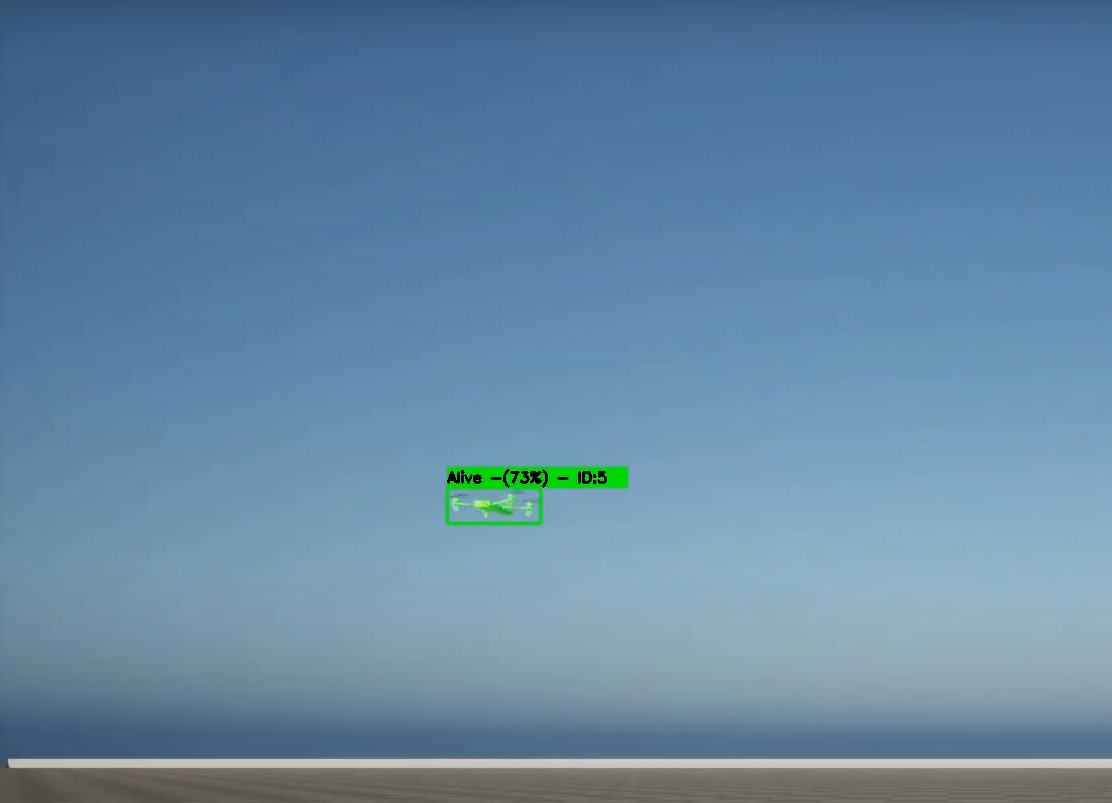
\includegraphics[width=.75\textwidth]{./Figures/deteccion_ejemplo.png}
\caption{Ejemplo de seguimiento por color.}
\label{fig:deteccion_ejemplo}
\end{figure}

El rendimiento y la robustez de los algoritmos de detección dependen en gran medida de la calidad y diversidad de los datos de entrenamiento. Por esta razón, se adopta una estrategia híbrida para la generación del conjunto de datos, combinando:
\begin{itemize}
    \item \textbf{Imágenes reales:} Capturadas en diversos escenarios y condiciones, representando fielmente el dominio de operación.
    \item \textbf{Imágenes sintéticas:} Generadas mediante el entorno de simulación desarrollado en Unreal Engine 5. Esta aproximación permite crear una gran variedad de situaciones, ángulos de visión, condiciones de iluminación y modelos de drones, superando las limitaciones logísticas y de costo asociadas a la recolección exclusiva de datos reales.
\end{itemize}

Un aspecto crítico en el entrenamiento de modelos de aprendizaje profundo es el fenómeno del \textit{overfitting}, donde el modelo aprende patrones específicos del conjunto de entrenamiento que no generalizan bien a datos nuevos. Para mitigar esto, se emplean técnicas de regularización como \textit{dropout}, aumento de datos (\textit{data augmentation}) y la mencionada incorporación de datos sintéticos, que enriquecen la variabilidad del conjunto de entrenamiento. Además, se considera el problema del desbalance de clases, ya que en escenarios reales los drones hostiles pueden ser menos frecuentes que otros objetos, lo que requiere estrategias como el muestreo ponderado o métricas de evaluación específicas como el F1-score.

\section{Mapeo}
El mapeo es el proceso mediante el cual un robot construye una representación espacial del entorno que lo rodea. Esta representación es fundamental para la navegación autónoma, permitiendo al robot localizarse a sí mismo y planificar rutas hacia un objetivo. En este proyecto, el robot está equipado con un sensor LIDAR (Light Detection and Ranging), que proporciona mediciones precisas de distancia a los objetos circundantes en forma de una nube de puntos.

\begin{figure}[htbp]
\centering
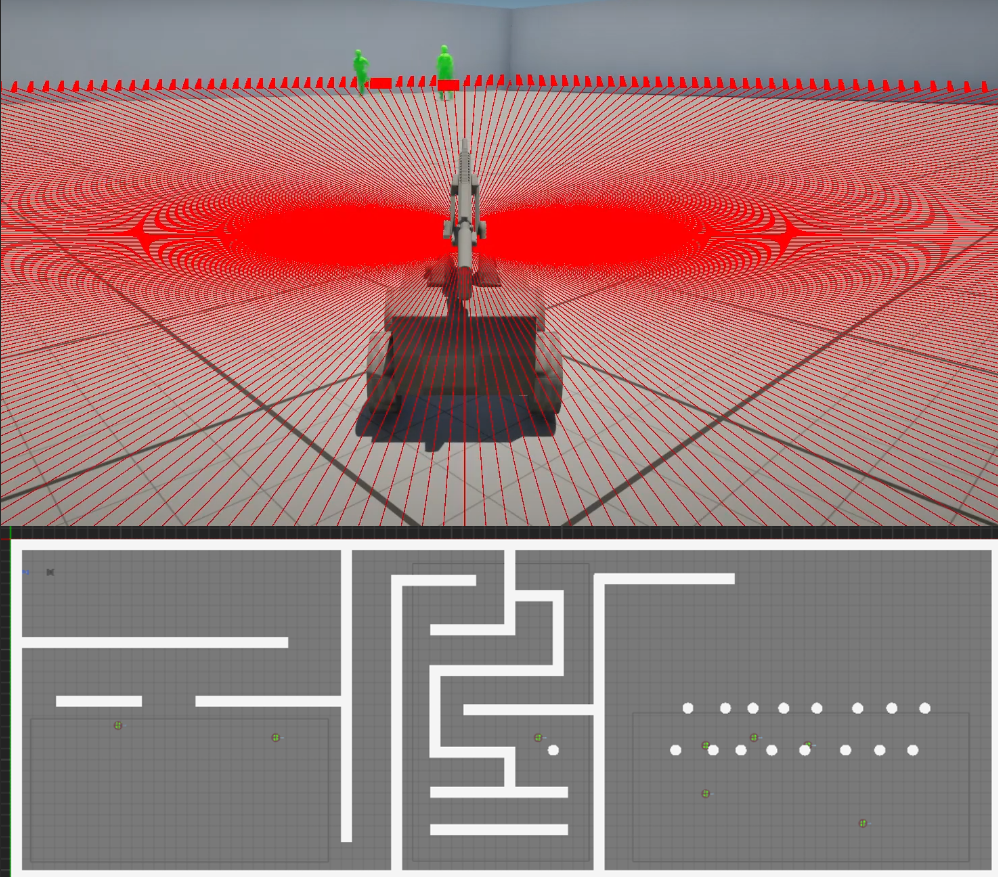
\includegraphics[width=.75\textwidth]{./Figures/mapeo_lidar_slam.png}
\caption{Ilustración del proceso de mapeo con LIDAR y SLAM.}
\label{fig:mapeo_lidar_slam}
\end{figure}

Para construir el mapa a partir de los datos del LIDAR y, simultáneamente, estimar la pose (posición y orientación) del robot dentro de ese mapa, se recurre a técnicas de SLAM (Simultaneous Localization and Mapping). El SLAM es un problema complejo, ya que la estimación de la pose del robot y la construcción del mapa son interdependientes. Desde un punto de vista teórico, el SLAM puede formularse como un problema de estimación bayesiana, donde se busca maximizar la probabilidad conjunta de la pose del robot y el mapa dado un conjunto de observaciones y controles. Esto implica modelar la incertidumbre inherente a las mediciones de los sensores y los errores acumulados en la odometría del robot.

Se investiga la aplicación de algoritmos eficientes de SLAM, con un enfoque particular en variantes como FastSLAM, que descompone el problema para mejorar la eficiencia computacional, especialmente en entornos de gran escala. FastSLAM utiliza un filtro de partículas para representar la incertidumbre en la pose del robot y mantiene estimaciones separadas para los \textit{landmarks} del entorno. Este enfoque combina las ventajas de los métodos basados en filtros de partículas con la eficiencia de los filtros de Kalman extendidos (EKF) para la estimación de \textit{landmarks}, reduciendo la complejidad computacional de $O(N^2)$ a $O(N \log M)$, donde $N$ es el número de partículas y $M$ el número de \textit{landmarks}. Además, se exploran enfoques más recientes como el SLAM basado en grafos (Graph-SLAM), que optimiza la trayectoria completa del robot y el mapa mediante la minimización de errores acumulados, siendo especialmente útil en entornos con bucles cerrados (\textit{loop closure}).

Un desafío adicional en el contexto militar es la operación en entornos dinámicos, donde objetos o personas pueden moverse, invalidando partes del mapa. Esto requiere la implementación de estrategias de actualización dinámica del mapa y la detección de cambios en el entorno, un área activa de investigación en el campo del SLAM.

\section{Path planning}
Una vez que el robot dispone de un mapa del entorno y conoce su ubicación, el siguiente paso es la planificación de rutas (path planning). Este proceso consiste en encontrar una trayectoria óptima o factible desde la posición actual del robot hasta un punto objetivo, evitando obstáculos y considerando otras restricciones (por ejemplo, el tipo de terreno o zonas prohibidas).

Para esta tarea, se implementa el algoritmo A* (A-star). A* es un algoritmo de búsqueda informada que encuentra el camino de menor costo entre un nodo inicial y un nodo objetivo en un grafo. Utiliza una función heurística para estimar el costo restante hasta el objetivo, lo que guía la búsqueda hacia las regiones más prometedoras del espacio de estados. Es ampliamente utilizado en robótica debido a su completitud (garantiza encontrar una solución si existe) y optimalidad (encuentra el camino de menor costo si la heurística es admisible). El mapa generado por el módulo SLAM sirve como base para la construcción del grafo sobre el cual opera A*.

Desde un punto de vista teórico, A* pertenece a la familia de algoritmos de búsqueda heurística y se deriva de la búsqueda de Dijkstra, pero incorpora una estimación del costo futuro (heurística) para priorizar los nodos a explorar. La función de evaluación de A* se define como $f(n) = g(n) + h(n)$, donde $g(n)$ es el costo acumulado desde el nodo inicial hasta el nodo $n$, y $h(n)$ es la heurística que estima el costo desde $n$ hasta el objetivo. Para garantizar la optimalidad, $h(n)$ debe ser admisible, es decir, nunca sobreestimar el costo real del camino restante. En este proyecto, se utiliza típicamente la distancia euclidiana o de Manhattan como heurística, dependiendo de la estructura del grafo que representa el mapa.

\begin{figure}[htbp]
\centering
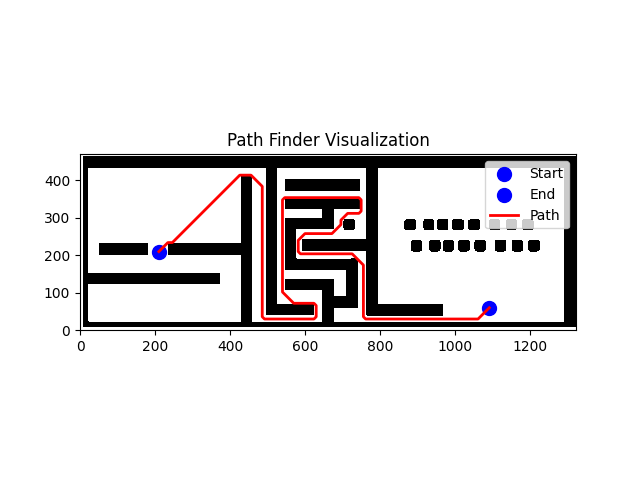
\includegraphics[width=.75\textwidth]{./Figures/path_planning_astar.png}
\caption{Ejemplo de planificación de ruta utilizando el algoritmo A*.}
\label{fig:path_planning_astar}
\end{figure}

Además de A*, existen otros enfoques para la planificación de rutas, como los algoritmos probabilísticos (por ejemplo, RRT - Rapidly-exploring Random Tree) que son más adecuados para espacios de alta dimensionalidad o entornos con obstáculos complejos. Sin embargo, A* se selecciona por su simplicidad de implementación y su eficacia en mapas discretizados, como los generados por SLAM. Un aspecto a considerar es la suavización de la trayectoria resultante, ya que A* puede generar caminos con cambios abruptos de dirección, no ideales para la dinámica de un robot físico. Para ello, se pueden aplicar técnicas de post-procesamiento como la interpolación de splines o algoritmos de suavizado basados en gradientes.

\section{Seguimiento de ruta}
Tras la planificación de una ruta, el robot debe ser capaz de seguirla con precisión. El seguimiento de ruta, también conocido como control de trayectoria o \textit{path tracking}, implica la implementación de algoritmos de control que ajustan continuamente los actuadores del robot (por ejemplo, velocidad y dirección de las ruedas o propulsores) para minimizar el error entre la posición actual del robot y la trayectoria deseada.

Existen diversas estrategias para el seguimiento de ruta, como los controladores PID (Proporcional-Integral-Derivativo), algoritmos de \textit{Pure Pursuit}, o técnicas basadas en modelos predictivos. La elección del controlador adecuado depende de la dinámica del robot, las características del entorno y los requisitos de precisión de la misión. El objetivo es asegurar que el robot se mantenga sobre la ruta planificada por A*, incluso ante perturbaciones o errores de estimación en su localización.

Teóricamente, el problema del seguimiento de ruta puede formularse como un problema de control óptimo, donde se busca minimizar una función de costo que representa el error de seguimiento y, potencialmente, otras variables como el consumo de energía o la suavidad del movimiento. Los controladores PID son una solución ampliamente utilizada debido a su simplicidad y robustez. Un controlador PID calcula la acción de control como una combinación lineal de tres términos: el error proporcional (P), la integral del error acumulado (I) para eliminar errores estacionarios, y la derivada del error (D) para anticipar cambios en el error. Sin embargo, los PID requieren un ajuste cuidadoso de sus parámetros (ganancias $K_p$, $K_i$, $K_d$) para cada sistema específico, lo que puede ser un proceso iterativo.

Por otro lado, el algoritmo \textit{Pure Pursuit} es un método geométrico que calcula un punto de mira (\textit{lookahead point}) en la trayectoria deseada, a una distancia fija del robot, y ajusta la dirección para alcanzarlo. Este enfoque es intuitivo y fácil de implementar, pero su desempeño depende críticamente de la elección de la distancia de anticipación, que debe balancear la estabilidad (distancias largas) con la precisión en curvas cerradas (distancias cortas). Finalmente, los controladores basados en modelos predictivos (MPC, Model Predictive Control) representan un enfoque más avanzado, donde se utiliza un modelo dinámico del robot para predecir su comportamiento futuro y optimizar las acciones de control en un horizonte de tiempo finito. Aunque computacionalmente más costoso, el MPC es capaz de manejar restricciones explícitas y dinámicas no lineales, siendo ideal para robots con comportamientos complejos.

\section{Simulación}
La simulación desempeña un papel fundamental en el desarrollo y validación de sistemas robóticos complejos, especialmente aquellos destinados a operar en entornos dinámicos o peligrosos. Permite probar algoritmos, evaluar diseños y realizar experimentos de forma segura, rápida y económica antes de realizar pruebas en el hardware físico.

Como se detalló en la Sección \ref{sec:simulador} , este proyecto utiliza Unreal Engine 5 (UE5) como plataforma de simulación. La elección de UE5 se justifica por su capacidad para generar entornos 3D realistas, simular físicas complejas y emular sensores como cámaras y LIDAR con alta fidelidad. Esto es esencial para:
\begin{itemize}
    \item Validar los algoritmos de percepción (detección de imágenes, SLAM).
    \item Probar y refinar los algoritmos de planificación y seguimiento de ruta en diversos escenarios.
    \item Generar datos sintéticos para el entrenamiento de modelos de aprendizaje automático, como se mencionó anteriormente.
    \item Realizar pruebas de integración del sistema completo en un entorno controlado.
\end{itemize}
El uso de un simulador avanzado como UE5 acelera significativamente el ciclo de desarrollo, permite la exploración de un mayor número de escenarios y contribuye a la robustez general del sistema robótico.

Desde una perspectiva teórica, la simulación en robótica se basa en la creación de modelos matemáticos y computacionales que aproximan el comportamiento del mundo real. Esto incluye la modelización de la dinámica del robot (cinemática y dinámica), las interacciones con el entorno (colisiones, fricción) y el ruido de los sensores. Un desafío clave es el \textit{reality gap}, la discrepancia entre el comportamiento simulado y el real, que puede limitar la transferibilidad de los resultados de la simulación al hardware físico. Para minimizar este problema, UE5 permite la incorporación de ruido sintético en las mediciones de los sensores y la simulación de condiciones ambientales variables, acercando el entorno virtual al real. Además, técnicas como el aprendizaje por transferencia (\textit{transfer learning}) y la adaptación al dominio (\textit{domain adaptation}) se utilizan para ajustar los modelos entrenados en simulación a datos del mundo real.
